\mysection{АНАЛИЗ ПРЕДМЕТНОЙ ОБЛАСТИ}

\subsection{Особенности работы GPS-приёмников}

Каждый GPS-приёмник определяет свои координаты, основываясь на расстояниях до спутников, с~которых он получает сигналы. Данные расстояния вычисляются из времени, которое требуется радиосигналам для прохождения от космических аппаратов до приёмника. \par

Для установления позиции приёмнику необходимо получать сигналы минимум от четырёх спутников. Каждый из этих сигналов может быть искажён при прохождении через слои атмосферы или при отражении от различных наземных объектов (рис.~\ref{fig:signal-distortion}) -- данные явления вызывают появление ошибок и~задержек, что отрицательно сказывается на точности позиционирования. \par

\begin{figure}[h!]
  \centering
  \setlength{\fboxsep}{5pt}
  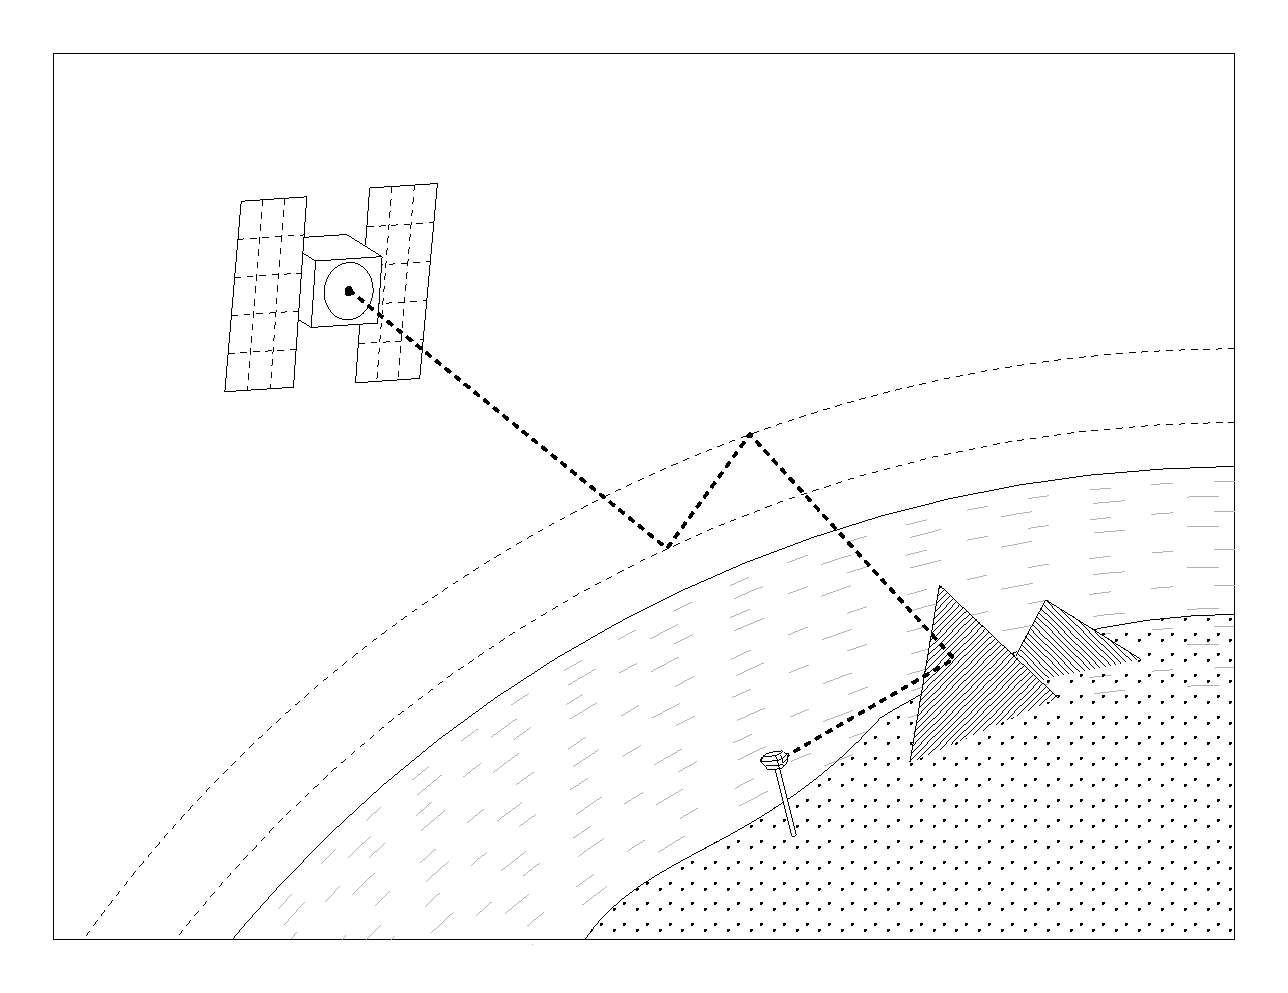
\includegraphics[height=8cm]{img/tikz/signal-distortion/pic}
  \caption{Источники ошибок: атмосферные задержки и~переотражение сигнала}\label{fig:signal-distortion}
\end{figure}

Важную роль в~решении проблемы, описанной выше, играет масштабность системы GPS. Расстояние между наземными объектами и~космическими спутниками так велико, что многие расстояния на земле становятся незначительными. Иными словами, если разместить два приёмника на расстоянии нескольких сотен километров друг от друга, то сигналы, которые они будут получать со~спутников, будут проходить практически через одну и~ту же часть атмосферы, что позволит считать ошибки на обоих приёмниках одинаковыми (рис.~\ref{fig:dgps-one}). \par

\begin{figure}[h!]
  \centering
  \setlength{\fboxsep}{5pt}
  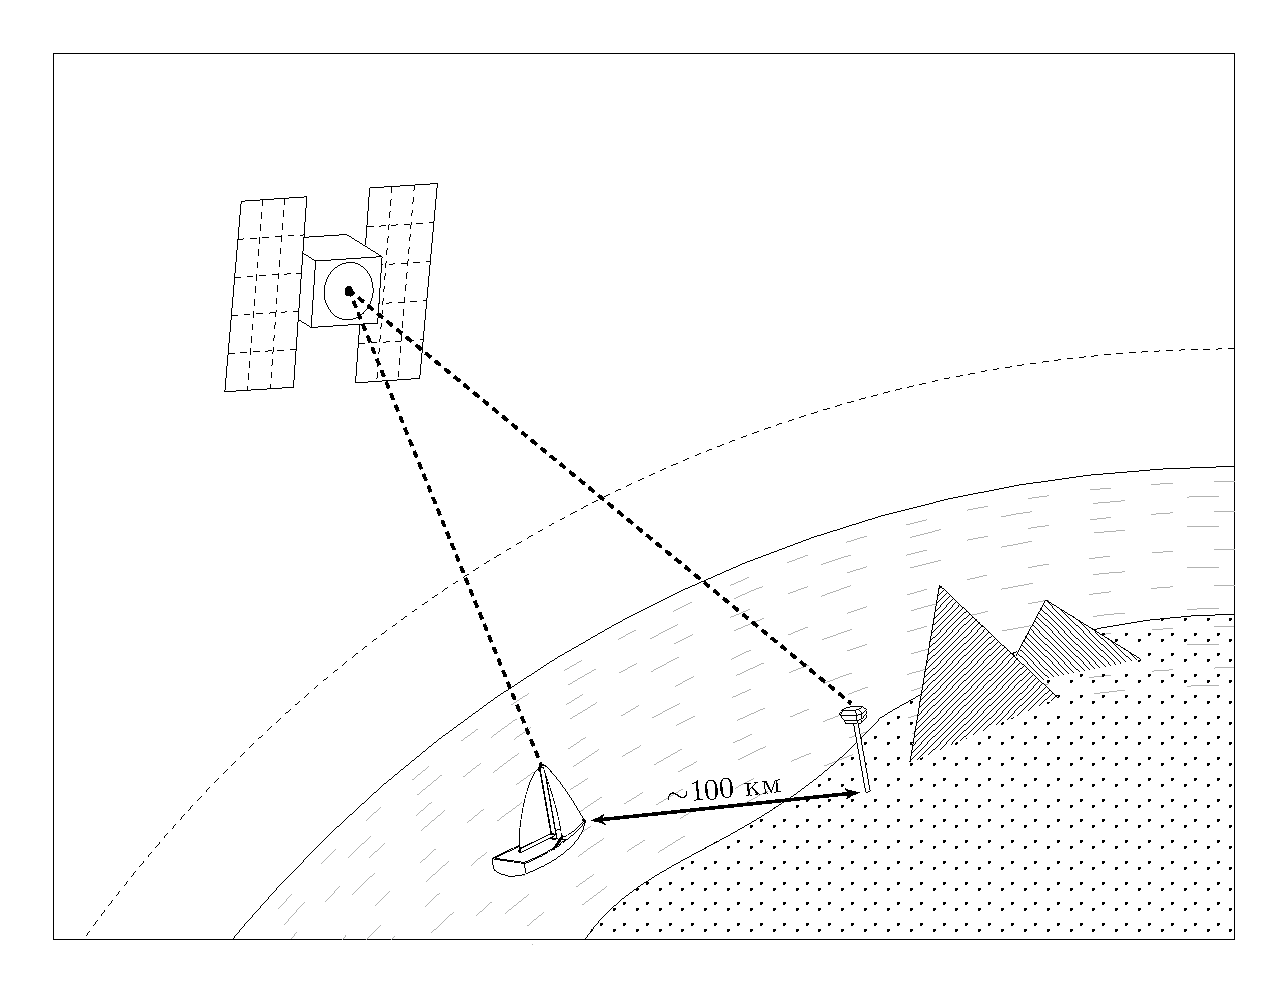
\includegraphics[height=8cm]{img/tikz/dgps-one/pic}
  \caption{База и~ровер, получающие сигналы с~одного спутника}\label{fig:dgps-one}
\end{figure}

Описанный выше принцип не является лишь теоретическими рассуждениями -- данный способ устранения ошибок применяется на практике и~является основой \emph{дифференциальной GPS}.

\subsection{Дифференциальная GPS и~кинематика реального времени}

\subsubsection{Дифференциальная GPS}

Дифференциальная GPS (англ. \emph{Differential Global Positioning System, DGPS}) -- система, предназначенная для повышения точности сигналов GPS. Принцип работы данной системы заключается в~измерении и~учёте разницы между рассчитанной и~закодированной псевдодальностями до спутников \cite{Trimble}. \par

Важнейшей особенность DGPS является использование двух приёмников при проведении измерений:

\begin{dashitemize}
  \item \textbf{База} (англ. \emph{base}) -- стационарный приёмник, который находится в~точке с~заранее рассчитанной координатой. База транслирует данные о~разнице между информацией о~позиции, полученной со~спутника, и~закодированными данными о~своём местонахождении.
  \item \textbf{Ровер} (англ. \emph{rover}) -- приёмник, с~помощью которого производятся какие-либо измерения. Используя данные, полученные с~базы, ровер учитывает влияние внешних факторов на расчёт координаты, тем самым получая более точную информацию о~своём местонахождении.
\end{dashitemize}

Таким образом, работа дифференциальной GPS основана на следующем принципе: считая искажения спутниковых сигналов одинаковыми для близлежащих приёмников, мы получаем возможность вносить поправки в~получаемое решение, улучшая результаты измерений.

\subsubsection{Кинематика реального времени}

Кинематика реального времени (англ. \emph{Real Time Kinematic, RTK}) -- режим работы, при котором приём и~применение поправок с~базы происходят в~реальном времени, что позволяет получать результат практически сразу. Важнейшей особенностью данного режима является тот факт, что для обеспечения работы необходима постоянная связь между ровером и~базой. \par

RTK представляется крайне удобным инструментом для задач, решение которых подразумевает использование высокоточного позиционирования. Однако, алгоритмы дифференциальной GPS, обеспечивающие работу RTK, весьма сложны, и~производители приёмников предлагают решение в~виде закрытого, проприетарного программного обеспечения, встроенного в~их продукты. Стоимость приёмников, поддерживающих дифференциальный режим работы, достаточно высока и~может превышать $10000$ долларов США. \par

Высокая стоимость оборудования является причиной того, что использование технологии дифференциальной GPS распространено только в~таких специфических областях деятельности, как геодезия, земельный кадастр и~т.п. Однако, для тех людей, которым по каким-либо причинам недоступны дорогостоящие устройства, решением может стать RTKLIB -- программный комплекс, реализующий вышеупомянутые алгоритмы для стандартных, общедоступных GPS-приёмников.

\subsection{Программный пакет RTKLIB}

RTKLIB -- программный пакет с~открытым исходным кодом, предназначенный для осуществления стандартного и~высокоточного позиционирования с~помощью ГНСС (глобальных навигационных спутниковых систем). В~состав пакета входит библиотека функций и~ряд приложений, использующих данную библиотеку. \par

Создателем RTKLIB является Томодзи Такасу, профессор Токийского Университета Морских Наук и~Технологий. Существенный вклад в~кодовую базу проекта был внесён Мишелем Баваро \cite{RTKLIB,Bavaro}, итальянским инженером с~огромным опытом работы в~сфере спутниковой навигации. \par

Начиная с~релиза первой версии RTKLIB, состоявшегося в~2007 году, проект активно развивается и~на данный момент представляет собой систему из восьми приложений, некоторые из которых имеют как графический, так и~консольный интерфейс. \par

Функции компонентов RTKLIB подробно описаны в~прилагающейся к~проекту официальной документации. Ниже будут рассмотрены наиболее важные для данной работы возможности программного комплекса.

\subsubsection{Поддерживаемые спутниковые системы}

RTKLIB поддерживает работу с~шестью основными системами спутниковой навигации:

\begin{dashitemize}
  \item GPS;
  \item GLONASS;
  \item Galileo;
  \item QZSS;
  \item BeiDou;
  \item SBAS.
\end{dashitemize}

Основной системой, позволяющей осуществлять высокоточное позиционирование является GPS. Остальные системы, как правило, служат источником дополнительных данных, которые помогают опровергнуть или подтвердить получаемое решение.

\subsubsection{Режимы работы}

Программный комплекс RTKLIB поддерживает несколько режимов работы, каждый из которых предназначен для решения различных навигационных задач. При выборе того или иного режима процесс работы с~приёмником может измениться коренным образом. Рассмотрим особенности и~назначение основных режимов работы комплекса:

\begin{dashitemize}
  \item \textbf{Single}, или \textbf{Single point positioning} (рис.~\ref{fig:rtk-single}). Базовый режим работы, при использовании которого можно получить координаты со~стандартной точность. В~режиме Single местоположение определяется с~помощью данных одного приёмника -- база в~данном режиме не используется. \par
  
  \begin{figure}[h!]
    \centering
    \setlength{\fboxsep}{5pt}
    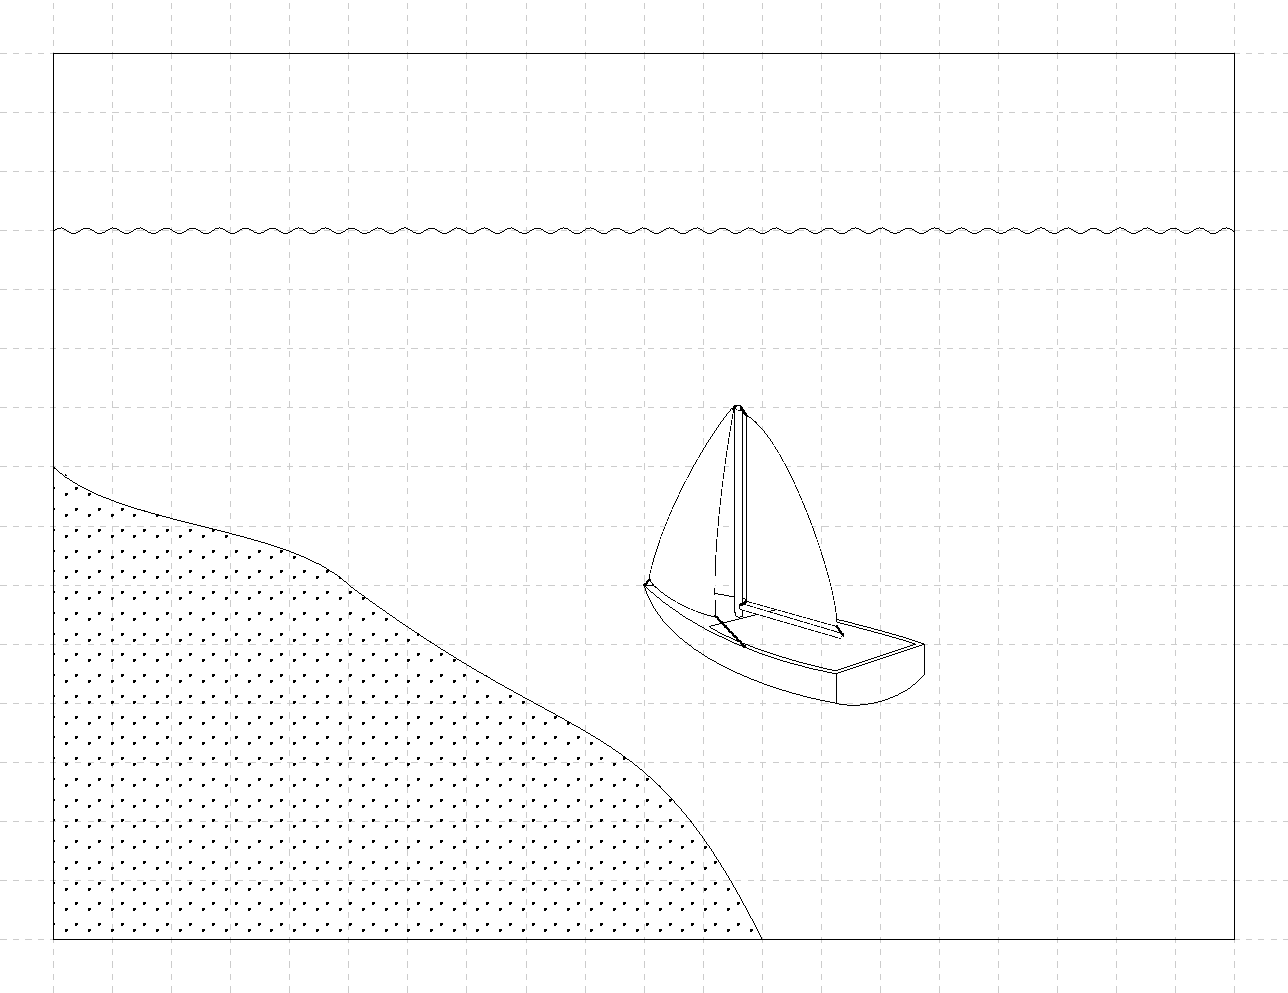
\includegraphics[height=8cm]{img/tikz/rtk-single/pic}
    \caption{Режим Single. Корабли, исполняющие роли роверов, не используют поправки с~базы, которая установлена на берегу}\label{fig:rtk-single}
  \end{figure}

  При использовании режима Single RTKLIB производит расчёт координаты, используя данные о~спутниках навигационной системы. Однако, сами приёмники, как правило, берут на себя задачу расчёта местоположения, т.к. они изначально оптимизированы для получения single-решения. \par
  RTKLIB в~режиме Single используется только на приёмниках, которые поддерживают функцию выдачи необработанных (или <<сырых>>) данных: фазовых измерений, псевдодальностей и~т.д. При работе в~данном режиме RTKLIB создаёт файлы логов <<сырых>> данных, которые далее можно будет использовать для постобработки (англ. \emph{post-processing}).
  
  \item \textbf{Static} и~\textbf{Kinematic} (рис.~\ref{fig:rtk-static-kinematic}). При данных настройках RTKLIB позволяет перейти от постобработки накопленных логов к~измерениям в~режиме реально времени (RTK). В~режимах Static и~Kinematic данные ровера используются вместе данными базовой станции, что позволит определять позицию ровера гораздо точнее. \par
  Отличием между режимами Static и~Kinematic является подвижность ровера. Если при работе в~режиме Static ровер считается неподвижным, то в~режиме Kinematic ровер находится в~движении. \par
  
  \begin{figure}[h!]
    \centering
    \setlength{\fboxsep}{5pt}
    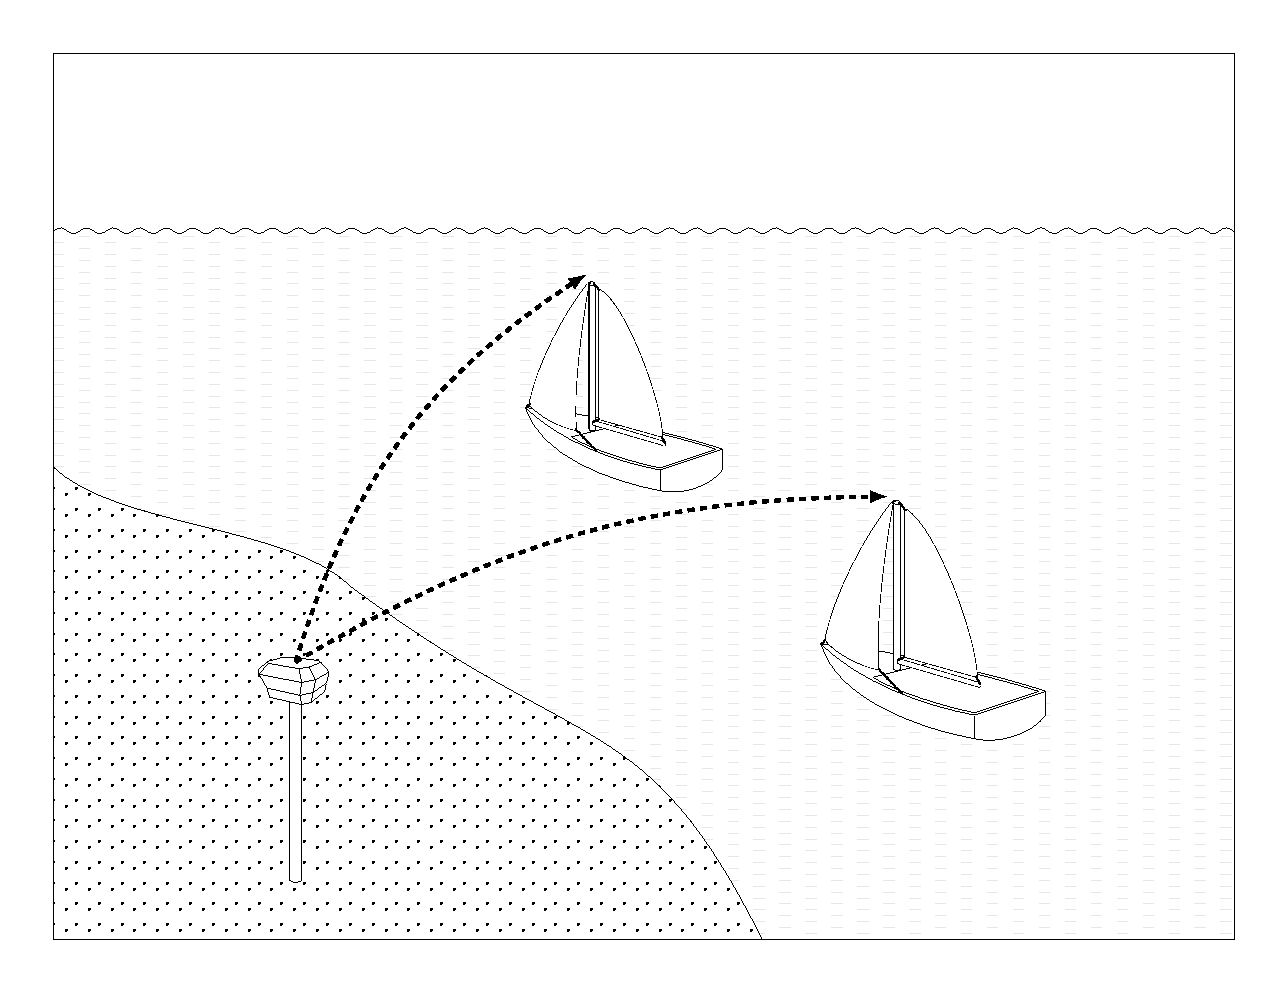
\includegraphics[height=8cm]{img/tikz/rtk-static-kinematic/pic}
    \caption{Режимы Static и~Kinematic. Корабли, исполняющие роли роверов, используют поправки с~базы, которая установлена на берегу}\label{fig:rtk-static-kinematic}
  \end{figure}
  
  Как и~в~случае Single, в~рассматриваемых режимах RTKLIB позволяет записывать логи необработанных данных ровера, однако важно отметить, что параллельно с~этим можно также вести лог поправок, получаемых с~базы. Сбор всех этих данных может быть крайне полезен для определения и~решения проблем связи между двумя приёмниками.
  
  \item \textbf{Moving-Baseline} (рис.~\ref{fig:rtk-moving-baseline}). Данный режим очень похож на Kinematic, но имеет одно ключевое отличие -- движущуюся базу. Moving-Baseline не предназначен для улучшения точности абсолютного позиционирования, однако относительно друг друга база и~ровер будут получать крайне точные координаты -- работая в~этом режиме, можно получить аналог GPS компаса.
  
  \begin{figure}[h!]
    \centering
    \setlength{\fboxsep}{5pt}
    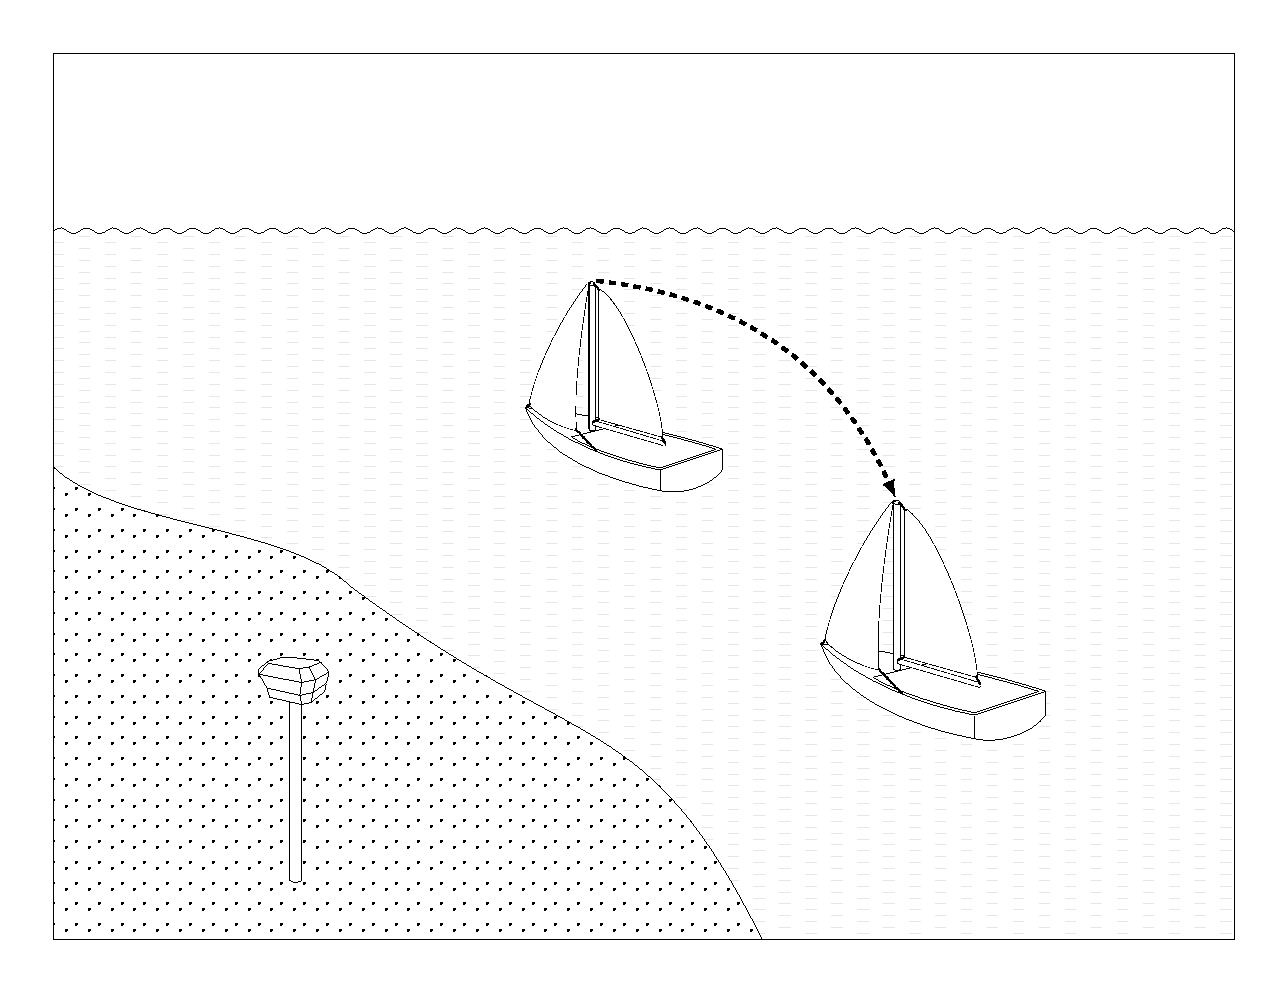
\includegraphics[height=8cm]{img/tikz/rtk-moving-baseline/pic}
    \caption{Режим Moving-Baseline. Один из кораблей выполняет роль базы и~передаёт поправки на корабль-ровер; оба корабля находятся в~движении}\label{fig:rtk-moving-baseline}
  \end{figure}
  
  \item \textbf{Precise point positioning}, или \textbf{PPP}. Режимы работы (PPP-Static, PPP-Kinematic и~PPP-Fixed), которые используются для подготовке к~работе в~режиме RTK. \par
  Среди перечисленных выше PPP режимов интерес для данной работы представляет PPP-Static, который используется для определения позиции будущей базы. Суть работы RTKLIB при таких настройках заключается в~накоплении и~усреднении информации о~текущей позиции приёмника. Проработав таким образом в~одной точке несколько часов, приёмник может с~хорошей степенью точности определить координаты своего местоположения и~выдать данные для настройки базы.
\end{dashitemize}

\subsubsection{Поддерживаемые форматы данных}

RTKLIB поддерживает множество форматов хранения данных, используемых при работе с~ГНСС. Набор поддерживаемых форматов включает в~себя как независимые от специфических устройств форматы (стандартные форматы), так и~форматы, используемые для выдачи координат лишь GPS-приём-никами определённых производителей (проприетарные форматы). \par

Стандартные форматы сообщений:
\begin{dashitemize}
  \item RINEX (сокр. англ. \emph{Receiver Independent Exchange Format});
  \item RTCM (сокр. англ. \emph{Radio Technical Commission for Maritime Services});
  \item NMEA (сокр. англ. \emph{National Marine Electronics Association}).
\end{dashitemize}

Примеры поддерживаемых проприетарных форматов сообщений:
\begin{dashitemize}
  \item UBX (приёмники u-blox);
  \item NovAtel;
  \item Hemisphere;
  \item JAVAD;
  \item Furuno;
  \item NVS.
\end{dashitemize}

\subsubsection{Программы, входящие в~состав RTKLIB}

Для понимания внутреннего устройства и~получения представления о~функциональности различных компонентов RTKLIB, следует рассмотреть программы, входящие в~состав данного программного пакета. Как уже было сказано ранее, последние версии RTKLIB -- 2.4.2 и~2.4.3 beta -- включают в~себя восемь приложений, отвечающих за различные функции комплекса. \par

В~рамках данной работы рассматриваются три приложения RTKLIB, отвечающие за ключевые функции, необходимые при решении задач навигации и~позиционирования: RTKNAVI, STRSVR и~RTKCONV.

\begin{dashitemize}
  \item \textbf{RTKNAVI} -- программа, обеспечивающая работу приёмника в~режиме RTK. RTKNAVI выполняет все задачи, возлагаемые на ровер:
  \begin{dashitemize}
    \item приём необработанных данных с~GPS-приёмника;
    \item приём поправок с~базы;
    \item ведение логов полученных данных;
    \item обработка данных с~помощью RTK алгоритмов;
    \item выдача полученного решения в~указанном формате.
  \end{dashitemize}

  Также, с~помощью RTKNAVI пользователь получает наглядную информацию о~качестве текущего решения и~о~сигналах, получаемых ровером и~базой со~спутников. \par
  
  RTKNAVI имеет консольный аналог -- приложение под названием \textbf{RTKRCV}. Текстовое версия поддерживает все функции графического приложения, включая вывод информации о~решении, спутниках и~текущих координатах. \par
  Важным отличием двух вариантов приложения является способ установки настроек -- если RTKRCV имеет отдельное окно с~графическими элементами управления, то RTKRCV настраивается только с~помощью конфигурационных файлов, работа с~которыми требует от пользователя определённых навыков.
  
  \item \textbf{STRSVR} является мультиплексором потоков данных, который позволяет создать до трёх каналов передачи связи, в~которые будет направлен вывод подключённого к~компьютеру GPS-приёмника. \par
  STRSVR предоставляет широкий набор возможностей по перенаправлению данных:
  
  \begin{dashitemize}
    \item передача через COM-порты;
    \item передача через TCP сокеты;
    \item передача через NTRIP-серверы;
    \item запись в~файл.
  \end{dashitemize}

  Также STRSVR обеспечивает (для каждого из выходных потоков) конвертацию входящих данных в~указанный пользователем формат. Только STRSVR может осуществлять выдачу информации в~легковесном формате RTCM3, что необходимо для обеспечения работы в~режиме базы. \par
  
  Консольная версия данного приложения носит название \textbf{STR2STR}.
  
  \item \textbf{RTKCONV}, или его консольный аналог \textbf{CONVBIN} -- конвертер данных, получаемых со~спутников. Одно из самых важных применений данной программы -- конвертация файлов логов из форматов, привязанных к~конкретным приёмникам, в~независимый формат RINEX. \par
  
  Использование RTKCONV может быть обусловлено необходимостью проведения дальнейшего анализа и~постобработки данных с~использованием специального программного обеспечения.
\end{dashitemize}

\subsection{Основные проблемы использования RTKLIB}

RTKLIB предоставляет широчайший спектр возможностей, а~исходный код данного проекта является открытым. Однако, данный комплекс распространён достаточно слабо и~не является широко известным. Данный факт связан отнюдь не с~низким качеством результатов работы RTKLIB, а, в~первую очередь, с~удобством использования данного программного продукта. \par

Графические версии приложений RTKLIB возможно запустить только в~среде операционной системы семейства Windows. Однако, достаточно проблематично обеспечить запуск графических Windows-приложений, к~примеру, на беспилотном летательном аппарате или на ГНСС-приёмнике. Но полностью раскрыть потенциал RTK можно именно при интеграции программного обеспечения в~технику. Данный факт делает консольные версии программ RTKLIB более привлекательным вариантом. \par

Входящие в~состав пакета текстовые приложения не требуют больших вычислительных ресурсов и~могут быть запущены на огромном количестве платформ под управлением GNU/Linux. Но важно понимать, что для работы с~консольными приложениями необходимо постоянно поддерживать работу одного или нескольких терминалов, а~также иметь компьютер с~клавиатурой и~доступом к~данным приёмника. \par

Вне зависимости от того, используются ли графические или консольные версии приложений, невозможно использовать обширные возможности RTKLIB без знания особенностей процесса конфигурирования данного комплекса. Огромное количество настроек вкупе с~различными режимами работы могут вызвать трудности при освоении RTKLIB новыми пользователями, а~разнообразные конфигурационные файлы и~неочевидные с~первого взгляда решения в~дизайне графических настроек способны запутать даже опытных пользователей.

Таким образом, можно выделить следующий ряд трудностей, которые могут возникнуть при использовании RTKLIB:

\begin{dashitemize}
  \item работа с~комплексом возможна только при наличии компьютера с~клавиатурой;
  \item графические приложения, входящие в~состав пакета, можно запустить только при использовании операционной системы семейства Windows;
  \item конфигурационные файлы консольных версий программ имеют достаточно сложный синтаксис;
  \item большое количество доступных настроек может затруднить освоение комплекса новыми пользователями.
\end{dashitemize}

В~качестве решения проблем, перечисленных выше, данная работа предлагает создать веб-приложение, с~помощью которого можно было бы осуществлять контроль над работой RTKLIB, используя практически любое устройство с~веб-браузером. Работа подобного приложения будет обеспечиваться с~помощью дополнительного программного обеспечения, добавленного на вычислительный модуль, на котором запущен RTKLIB. Осуществляя с~помощью такого программного обеспечения обмен командами и~информацией между веб-интерфейсом и~RTKRCV, можно осуществлять работу с~RTKLIB, используя смартфон или планшет.

\subsection{Обзор существующих веб-приложений, предназначенных для работы с~устройствами без органов управления}

\subsection{Выводы по разделу 1}

\newpage
